\chapter{Teoretická část}

\section{Problém obchodního cestujícího}
Problém obchodního cestujícího patří mezi nejznámější úlohy kombinatorické optimalizace. Jedná se o permutační problém, jehož cílem je nalézt nejkratší uzavřenou cestu, která navštíví množinu zadaných lokalit právě jednou a vrátí se do výchozího bodu. \cite{jancar_vsb_ti_skript}.

\subsection{Formální definice problému}
% https://www.cs.vsb.cz/sawa/uti/2025/slides/uti-cz.pdf | 21 slide

Matematicky lze TSP modelovat pomocí teorie grafů. Pro zajištění obecnosti, která zahrnuje i \textbf{asymetrické instance}, definujeme problém na orientovaném grafu. 

Nechť $G = (V, A)$ je úplný orientovaný graf, kde $V = \{v_1, v_2, \dots, v_n\}$ je množina $n$ vrcholů a $A = \{(i, j) : i, j \in V, i \neq j\}$ je množina orientovaných hran. Každé hraně $(i, j)$ je přiřazena nezáporná váha $c_{ij}$, která reprezentuje cenu přesunu (vzdálenost, čas či energii) z vrcholu $i$ do vrcholu $j$. V závislosti na vlastnostech matice cen $\mathbf{C}$ rozlišujeme dvě základní varianty:
\begin{itemize}
    \item \textbf{Symetrické TSP:} Pro všechny dvojice vrcholů platí $c_{ij} = c_{ji}$.
    \item \textbf{Asymetrické TSP:} Existuje alespoň jedna dvojice $(i, j)$ taková, že $c_{ij} \neq c_{ji}$.
\end{itemize}

Cílem je nalézt takovou permutaci $\pi$ indexů $\{1, \dots, n\}$, která minimalizuje celkovou nákladovou funkci~\cite{reinelt1994tsplib}:

\begin{equation}
    \min z(\pi) = \sum_{i=1}^{n-1} c_{\pi(i), \pi(i+1)} + c_{\pi(n), \pi(1)}
\end{equation}

Kde jednotlivé členy výrazu reprezentují:
\begin{itemize}
    \item $\pi$ je konkrétní permutace indexů vrcholů z množiny všech přípustných řešení.
    \item $c_{\pi(i), \pi(i+1)}$ vyjadřuje náklady na přesun z vrcholu na $i$-té pozici do vrcholu na pozici $(i+1)$ v daném pořadí $\pi$.
    \item Člen $c_{\pi(n), \pi(1)}$ zajišťuje uzavření cyklu, tedy započtení cesty z posledního navštíveného vrcholu zpět do vrcholu výchozího.
\end{itemize}

Tato uzavřená cesta, která navštíví každý vrchol grafu právě jednou, se v teorii grafů nazývá \textbf{Hamiltonovský cyklus}. V informatice lze vrcholy a hrany reprezentovat maticí sousednosti (vzdáleností) $\mathbf{C} = [c_{ij}]_{n \times n}$, kde jednotlivé prvky představují váhy hran mezi dvojicemi vrcholů $v_i$ a $v_j$. Tato reprezentace umožňuje efektivní algoritmické zpracování stavového prostoru a je základem pro většinu implementací heuristických i exaktních algoritmů.

\begin{equation}
\label{eq:general_cost_matrix}
C = 
\begin{pmatrix}
c_{11} & c_{12} & \cdots & c_{1n} \\
c_{21} & c_{22} & \cdots & c_{2n} \\
\vdots & \vdots & \ddots & \vdots \\
c_{n1} & c_{n2} & \cdots & c_{nn}
\end{pmatrix}
\end{equation}

\subsection{Ilustrace problému a řešení}

Pro lepší pochopení podstaty TSP je vhodné interpretovat instanci graficky. Obrázek \ref{fig:neoptimalni_tsp} ukazuje neoptimalizovaný stav a obrázek \ref{fig:optimalni_tsp} ukazuje nalezené přípustné řešení po aplikaci optimalizačního algoritmu.

\begin{itemize}
    \item \textbf{Neoptimalizovaná instance:} Představuje náhodné nebo abecední seřazení lokalit, které má obchodní cestující navštívit. V grafickém znázornění je patrný vizuální chaos a velké množství křížících se hran. Celková délka takové trasy je z logistického hlediska neefektivní a představuje horní odhad nákladů.
    \item \textbf{Optimalizovaná instance:} Zobrazuje výsledek hledání Hamiltonovské kružnice s minimální (nebo blízkou minimální) celkovou délkou. V euklidovském prostoru je typickým znakem optima absence křížení hran a plynulé navazování cesty mezi geograficky blízkými uzly.
\end{itemize}

\begin{figure}[H]
  \centering
  \begin{minipage}[b]{0.4\textwidth}
    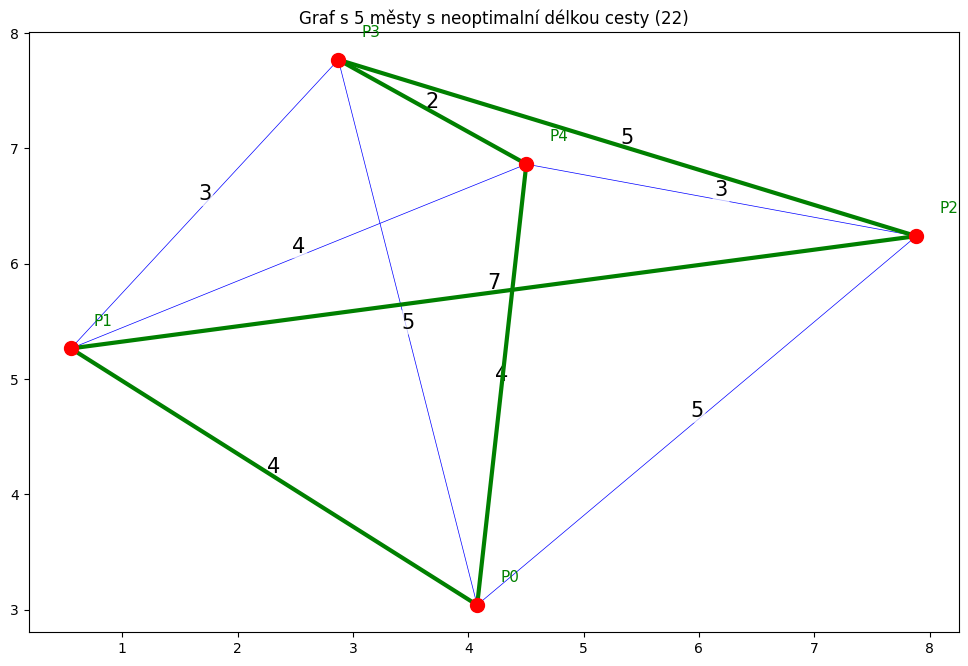
\includegraphics[width=\textwidth]{Figures/neoptimalni_tsp.png}
    \caption{Neoptimální instance}
    \label{fig:neoptimalni_tsp}
  \end{minipage}
  \hfill
  \begin{minipage}[b]{0.4\textwidth}
    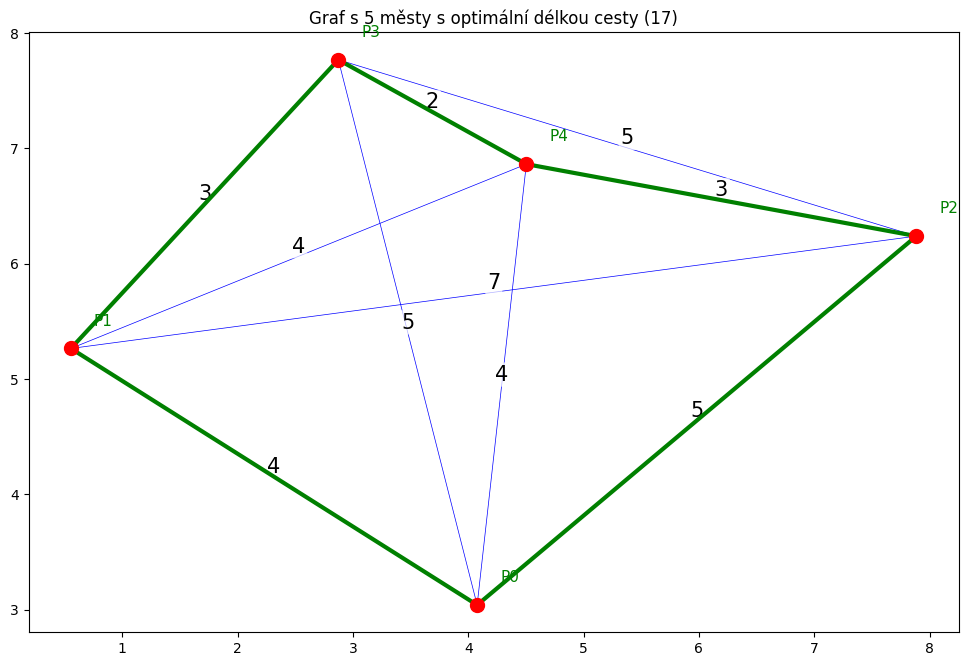
\includegraphics[width=\textwidth]{Figures/optimalni_tsp.png}
    \caption{Optimální instance}
    \label{fig:optimalni_tsp}
  \end{minipage}
\end{figure}

\subsection{Typy TSP}
Jak bylo definováno v předchozí části, základním datovým vstupem pro řešení problému je matice vzdáleností $\mathbf{C}$, kde prvek $c_{ij}$ reprezentuje ohodnocení hrany mezi uzly $v_i$ a $v_j$. V závislosti na vnitřních vlastnostech této matice a charakteru reálného prostředí, které má generátor simulovat, rozlišujeme následující varianty:

\begin{itemize}
    \item \textbf{Symetrický TSP (STSP):} Tato varianta předpokládá, že matice $\mathbf{C}$ je symetrická podle hlavní diagonály, tedy platí $c_{ij} = c_{ji}$ pro všechna $i, j \in V$. V praxi to znamená, že náklady na cestu z bodu $A$ do bodu $B$ jsou identické jako v opačném směru. Tento model je typický pro euklidovské instance (např. typ \texttt{EUC\_2D} v TSPLIB \cite{reinelt1994tsplib,tsplib95}), kde se vzdálenosti mezi uzly obvykle odvozují z jejich souřadnic v rovině jako eukleidovské vzdálenosti (délka přímky spojující daný pár bodů).
    
    \item \textbf{Asymetrický TSP (ATSP):} Zde podmínka symetrie neplatí a v matici existuje alespoň jeden pár indexů, pro který $c_{ij} \neq c_{ji}$. Pro generátor využívající mapová API je tato varianta klíčová, neboť v reálné silniční síti jsou náklady na přesun ovlivněny jednosměrnými ulicemi, dálničními nájezdy nebo výškovým profilem trasy.
    
    \item \textbf{Metrický TSP (trojúhelníková nerovnost):} Jedná se o typ, kde prvky matice splňují trojúhelníkovou nerovnost: $c_{ij} \leq c_{ik} + c_{kj}$ pro libovolnou trojici vrcholů. U reálných silničních dat tato vlastnost závisí na volbě nákladové funkce a konkrétních omezeních dopravy. Nelze ji proto obecně předpokládat pro všechny typy výstupů mapových služeb.
    
    \item \textbf{Dynamický TSP:} Na rozdíl od statických matic v TSPLIB \cite{reinelt1994tsplib,tsplib95}, v této variantě je $c_{ij}$ funkcí času $c_{ij}(t)$. To umožňuje reflektovat proměnlivou dopravní situaci (např. dopravní špičky zjištěné přes API).
\end{itemize}


\subsection{NP-úplnost a výpočetní složitost}
Z hlediska teorie složitosti je nezbytné u TSP rozlišovat mezi jeho optimalizační a rozhodovací variantou. Optimalizační úloha, tedy hledání Hamiltonovské kružnice s minimálním součtem vah hran, spadá do třídy \textbf{NP-těžkých} (NP-hard) problémů. To znamená, že pro ni neexistuje známý algoritmus s polynomem omezenou časovou složitostí, pokud neplatí $P = NP$ \cite{reinelt1994tsplib}.

Rozhodovací verze TSP (označovaná jako \textit{TSP decision problem}) se ptá, zda v daném grafu $G$ existuje Hamiltonovská kružnice s celkovou váhou $c \leq k$ pro zadanou konstantu $k$. Konstanta $k$ je součástí vstupu úlohy. Představuje pevně zvolenou horní mez na součet vah hran kružnice. Odpověď je ano, pokud existuje Hamiltonovská kružnice, jejíž celková cena nepřekročí $k$, jinak ne. Tato varianta patří mezi \textbf{NP-úplné} problémy. Její náročnost lze dokázat polynomiální redukcí z problému Hamiltonovské kružnice (HC), který je jedním z klasických NP-úplných problémů \cite{jancar_vsb_ti_skript,reinelt1994tsplib}.
Výpočetní náročnost je dána explozivním růstem stavového prostoru. 

Počet přípustných řešení roste faktoriálně. U asymetrického TSP zafixujeme počáteční vrchol a zbylých $n-1$ vrcholů můžeme uspořádat libovolně, proto je počet různých cest $(n-1)!$. U symetrického TSP každá taková cesta odpovídá stejné kružnici i při opačném směru průchodu, takže počet různých kružnic je poloviční:
\begin{equation}
    \frac{(n-1)!}{2}
\end{equation}
\cite{reinelt1994tsplib}.
Tento faktoriální růst způsobuje, že i pro relativně malé instance (např. $n=20$) je nalezení globálního optima metodou hrubé síly v reálném čase neproveditelné. Zatímco ověření kandidátního řešení (zda je cesta Hamiltonovská a zda její váha nepřekračuje $k$) je řešitelné v polynomiálním čase, samotné nalezení optima vyžaduje nasazení pokročilých heuristik nebo aproximačních algoritmů, kterým se věnuje kapitola \ref{subsection:BIA}.


\section{Stanovení vah hran v reálných sítích}
V klasických formulacích TSP se předpokládá, že váhy hran jsou již definovány. V rámci této práce, která se zaměřuje na generování instancí z reálných geografických dat, je však klíčovým krokem výpočet nejkratších cest mezi každou dvojicí lokalit v grafu silniční sítě. Tento proces předchází samotnému řešení TSP a využívá algoritmy pro hledání nejkratší cesty mezi dvěma body.

\subsection{Dijkstrův algoritmus}
Dijkstrův algoritmus je deterministický algoritmus pro hledání nejkratších cest z jednoho zdrojového uzlu do všech ostatních v grafu s nezápornými vahami hran. Algoritmus udržuje množinu navštívených uzlů a pro každý uzel si pamatuje aktuální nejkratší nalezenou cestu. V každém kroku expanduje uzel s minimální dosaženou vzdáleností \cite{dijkstra1959note}. V praxi routovacích enginů se pro zrychlení dotazů často používá kombinace s technikou \textit{Contraction Hierarchies}, která staví na modifikovaném obousměrném vyhledávání nejkratší cesty \cite{geisberger2008ch}. Konkrétně například OSRM nabízí předzpracování pomocí CH a službu \texttt{Table} pro výpočet matic vzdáleností či časů mezi zadanými body \cite{osrm_backend_readme}.


\subsection{Algoritmus A*}
A* je heuristicky řízené rozšíření vyhledávání nejkratší cesty, které používá hodnoticí funkci složenou z již známé ceny cesty a odhadu zbývající ceny do cíle \cite{hart1968astar}.
\begin{itemize}
    \item \textbf{Heuristika:} Na rozdíl od čistě nákladového prohledávání bez odhadu cíle využívá A* heuristickou složku, takže preferuje uzly, které podle odhadu vedou k cíli výhodněji \cite{hart1968astar}. V mapových úlohách se jako heuristika často používá vzdušná vzdálenost mezi uzlem a cílem.

\begin{equation}
\label{eq:a_star}
f(n) = g(n) + h(n)
\end{equation}
Tento tvar hodnoticí funkce je přímo uveden v původní práci o A*~\cite{hart1968astar} kde:
\begin{itemize}
    \item $g(n)$ představuje cenu nejlevnější dosud nalezené cesty ze startu do uzlu $n$ \cite{hart1968astar}.
    \item $h(n)$ je heuristický odhad zbývající ceny z uzlu $n$ do cíle \cite{hart1968astar}.
\item $f(n)$ je výsledná priorita uzlu. V každém kroku se rozšiřuje otevřený uzel s nejmenší hodnotou $f(n)$ \cite{hart1968astar}.
\end{itemize}
    \item \textbf{Význam:} V kontextu této práce je A* důležitý jako základní princip informovaného vyhledávání. V praktických routovacích enginech se nad velkými silničními grafy často používají i specializovaná zrychlení, například Contraction Hierarchies, případně alternativní pipeline typu MLD \cite{geisberger2008ch,osrm_backend_readme}.
\end{itemize}





\section{Metody řešení TSP}
Vzhledem k prokázané složitosti problému je volba metody řešení vždy kompromisem mezi výpočetním časem a kvalitou nalezeného řešení. Metody lze kategorizovat do čtyř hlavních skupin.

\subsection{Přesné metody}
Tyto algoritmy garantují nalezení teoretického globálního optima, avšak jejich časová složitost je v nejhorším případě exponenciální \cite{johnson1997tsp_local_search}.
\begin{itemize}
\item \textbf{Brute Force:} 
    Tento přístup spočívá v systematickém generování všech přípustných řešení, tedy všech možných Hamiltonovských kružnic v grafu. Algoritmus vypočítá délku každé takové trasy a vybere tu s minimální hodnotou.
    
    \textit{Složitost a limity:} Naivní úplné prohledání všech permutací měst má časovou složitost $O(n!)$ \cite{cmu_15451_dp2_2023}. Metoda je proto prakticky použitelná jen pro malé instance nebo pro validační účely.

    \item \textbf{Branch and Bound:} 
    Jedná se o metodu prohledávání stavového prostoru, která na rozdíl od hrubé síly neprochází všechny kombinace, ale ořezává ty části stromu řešení, které prokazatelně nemohou vést k optimu. V klasické formulaci pro TSP se množina všech tras postupně dělí na menší podmnožiny (branching) a pro každou se počítá dolní mez (bounding) \cite{little1963bnb}. Algoritmus využívá dvě základní operace:
    \begin{enumerate}
        \item \textbf{Větvení (Branching):} Rozdělení aktuálního problému na menší podproblémy (např. zahrnutí nebo vyloučení konkrétní hrany $e_{ij}$ z trasy).
        \item \textbf{Určování mezí (Bounding):} Pro každý uzel ve stromu výpočtu se určí dolní mez (lower bound) ceny řešení. Tato mez se často získává pomocí relaxace problému (např. řešením přiřazovacího problému nebo výpočtem minimální kostry grafu).
    \end{enumerate}
    
    Pokud je vypočtená dolní mez určité větve vyšší než cena doposud nejlepšího nalezeného řešení (\textit{upper bound}), je celá tato větev z dalšího prohledávání vyřazena \cite{little1963bnb}. 
    
    \textit{Výhody:} Při účinném prořezávání může výrazně snížit počet prozkoumaných stavů oproti úplnému výčtu.
    
    \textit{Nevýhody:} V nejhorším případě může být běh stále výpočetně prohibitivní \cite{lin1973tsp}.
    
\item \textbf{Dynamické programování (Bellman-Held-Karpův algoritmus):} 
Tento přístup využívá principu optimality, kdy optimální řešení celého problému lze sestavit z optimálních řešení jeho podproblémů. Na rozdíl od metod typu Branch and Bound, které prohledávají větve stromu a ořezávají je na základě mezí, Held-Karpův algoritmus systematicky buduje tabulku výsledků pro všechny možné podmnožiny měst \cite{nguyen2020bhk}.

\textit{Princip:} Nechť $S \subseteq V \setminus \{v_1\}$ je podmnožina měst a $g(v_i, S)$ je délka nejkratší cesty začínající v počátečním městě $v_1$, procházející všemi městy v $S$ právě jednou a končící v městě $v_i$. Algoritmus rekurzivně vypočítává hodnoty $g$ pro rostoucí velikost množiny $S$, přičemž využívá již vypočtené hodnoty uložené v paměti \cite{nguyen2020bhk}.

\textit{Složitost a limity:} Standardní formulace redukuje naivní $O(n!)$ na $O(n^2 2^n)$ \cite{nguyen2020bhk}. Počet stavů DP je řádově $n 2^n$, což v praxi vede k vysoké paměťové náročnosti při větších instancích \cite{nguyen2020bhk}.

\textit{Výhody:} Metoda poskytuje řešení deterministickým stylem, tedy bez závislosti na kvalitě prořezávání, která je typická pro Branch and Bound.

\textit{Nevýhody:} Nároky na čas i operační paměť rostou exponenciálně, takže u rozsáhlých logistických sítí je metoda obvykle prakticky limitující a častěji slouží jako referenční přesný přístup než jako nasazované produkční řešení \cite{nguyen2020bhk}.
\end{itemize}

\subsection{Heuristiky a lokální optimalizace}
Lokální optimalizace (označované také jako metody lokálního prohledávání) pracují na principu iterativního vylepšování již existujícího přípustného řešení. Cílem je najít v definovaném okolí aktuální trasy takovou změnu, která sníží celkovou cenu \cite{johnson1997tsp_local_search}.

\begin{itemize}
    \item \textbf{Algoritmy $k$-opt (2-opt a 3-opt)} \cite{johnson1997tsp_local_search}\textbf{:} Číslo $k$ definuje počet hran aktuálního cyklu, které jsou v jednom kroku odstraněny a následně nahrazeny jinou kombinací hran tak, aby byla zachována integrita Hamiltonovské kružnice.
    \begin{itemize}
    \item \textbf{Princip 2-opt (záměna dvou hran):} 
    Představme si aktuální trasu jako uzavřený řetězec. Algoritmus vybere dvě hrany, které nesousedí (tedy nemají společný uzel). Tyto dvě hrany odstraní, čímž se trasa rozpadne na dvě samostatné cesty. Aby vznikla nová souvislá Hamiltonovská kružnice, musí algoritmus tyto dva úseky znovu propojit, ale v jiném pořadí.
    Pokud byla původní cesta $[A \to B \to \dots \to C \to D]$, po odstranění hran $(A,B)$ a $(C,D)$ a následném křížovém propojení vznikne trasa $[A \to C \to \dots \to B \to D]$. 
    
    
    \textit{Geometrický význam:} Pokud se původní dvě hrany křížily, tato operace křížení odstraní. V eukleidovských instancích vede odstranění křížení typicky ke zkrácení trasy. Nejde však o univerzální tvrzení pro libovolnou matici nákladů.
        \item \textbf{3-opt:} Tento přístup odstraňuje tři hrany současně, což umožňuje provádět mnohem komplexnější úpravy cesty (včetně přehození celých úseků trasy). Zatímco 2-opt dokáže najít pouze lokální optimum v rámci jednoduchých prohozů, 3-opt prohledává širší okolí řešení, což zvyšuje šanci na nalezení kvalitnější trasy, ovšem za cenu vyšší výpočetní náročnosti. Při úplném prohledání sousedství je ověření lokální optimality v nejhorším případě řádu $\Omega(n^2)$ pro 2-opt a $\Omega(n^3)$ pro 3-opt \cite{johnson1997tsp_local_search}.
\end{itemize}
    \item \textbf{Lin-Kernighan (LK):} Algoritmus Lin-Kernighan je v podstatě zobecněním $k$-opt přístupu, kde hodnota $k$ není předem fixně stanovena. Algoritmus v každém kroku adaptivně rozhoduje, kolik hran je vhodné zaměnit, a to na základě potenciálního zlepšení nákladové funkce. Díky této flexibilitě dokáže LK efektivně opustit lokální minima, ve kterých by se standardní 2-opt nebo 3-opt algoritmy zastavily. V praxi se často používá k dosažení řešení, která jsou velmi blízko optimu i pro instance s tisíci uzly \cite{lin1973tsp,helsgaun2000lk,helsgaun2009lkh}.
\end{itemize}

\subsection{Metaheuristiky a biologicky inspirované algoritmy}
\label{subsection:BIA}
Vzhledem k výpočetní náročnosti přesných metod se pro rozsáhlé instance moderní logistiky využívají metaheuristiky \cite{engelbrecht2002ci}. Tyto algoritmy nehledají globální optimum s absolutní jistotou, ale zaměřují se na nalezení dostatečně kvalitního řešení v akceptovatelném čase. Klíčovou vlastností těchto metod je schopnost unikat z lokálních optim pomocí mechanismů inspirovaných přírodou.

\begin{itemize}
    \item \textbf{Genetické algoritmy (GA):} Tato technika simuluje evoluční proces nad populací kandidátních řešení, kde noví potomci vznikají operacemi křížení a mutace \cite{engelbrecht2002ci,johnson1997tsp_local_search}. Pro TSP je zároveň nutné zachovat platnou permutaci měst, tedy bez opakované návštěvy stejného města \cite{johnson1997tsp_local_search}.
    
    \item \textbf{Mravenčí kolonie (Ant Colony Optimization - ACO):} ACO je inspirováno chováním reálných mravenců a pro TSP používá pravděpodobnostní volbu dalšího města podle feromonu a viditelnosti (inverzní vzdálenosti) \cite{dorigo1997acs}. Klíčovým mechanismem je vypařování feromonu a jeho následná aktualizace podle kvality nalezených tras, což umožňuje postupně zvýhodňovat lepší cesty \cite{dorigo1997acs}.
    
    \item \textbf{Simulované žíhání (Simulated Annealing - SA):} SA je definováno pomocí řídicích parametrů počáteční teploty, minimální teploty a chladicí konstanty. Přijímací pravidlo dovoluje s určitou pravděpodobností přijmout i horší řešení podle členu $e^{-(f(x_1)-f(x))/T}$, takže algoritmus na začátku více prozkoumává prostor řešení a s klesající teplotou se chová více lokálně.

    \item \textbf{Rat Swarm Optimizer (RSO):} Biologicky inspirovaný algoritmus, který simuluje inteligentní chování potkanů v hejnu během procesu lovu \cite{dhiman2021rso}. Algoritmus je strukturálně rozdělen do dvou klíčových fází:
\begin{itemize}
    \item \textbf{Fáze pronásledování (Chasing):} V této fázi se potkani pohybují směrem k lídrovi (nejlepšímu dosud nalezenému řešení). Matematicky je tento pohyb definován tak, aby agenti efektivně prohledávali okolí a balancovali mezi náhodným pohybem a následováním nejúspěšnějšího jedince. To umožňuje algoritmu pokrýt širokou oblast stavového prostoru a vyhnout se uvíznutí v lokálním optimu \cite{dhiman2021rso}.
    \item \textbf{Fáze boje (Fighting):} V kontextu TSP to znamená jemné ladění trasy v blízkosti nejlepšího nalezeného řešení. Tato fáze podporuje konvergenci algoritmu k finálnímu výsledku \cite{dhiman2021rso}.
\end{itemize}
Díky této kombinaci globálního prohledávání a lokálního zpřesňování dosahuje RSO dobrých výsledků i na komplexních instancích. Původní práce uvádí vyhodnocení na 38 benchmark funkcích. \cite{dhiman2021rso}.
\end{itemize}


\subsection{Aproximační a konstruktivní algoritmy}
Na rozdíl od běžných heuristik poskytují aproximační algoritmy pevnou matematickou garanci, která definuje maximální možnou odchylku nalezeného řešení od globálního optima \cite{reinelt1994tsplib}.
Tyto algoritmy jsou klíčové pro pochopení mezí výpočetní složitosti u metrických variant TSP.

\begin{itemize}
    \item \textbf{Nearest Neighbour:} 
    Tento algoritmus reprezentuje tzv. greedy přístup. Začíná v náhodně zvoleném uzlu a v každém dalším kroku se přesune do nejbližšího dosud nenavštíveného uzlu. Po navštívení všech měst se algoritmus vrátí do výchozího bodu. 
    
    \textit{Vlastnosti:} Je extrémně rychlý s časovou složitostí $O(n^2)$, avšak postrádá globální nadhled. Často se stává, že v závěru algoritmu zbývají uzly, které jsou od sebe velmi vzdálené, což vede k vytvoření neúměrně dlouhé závěrečné hrany.
    
    \item \textbf{Algoritmus založený na minimální kostře (MST):} 
    Pro instance splňující trojúhelníkovou nerovnost využívá tento přístup vlastností minimální kostry grafu. 
    
    \textit{Princip:} Nejdříve se sestrojí MST daného grafu. Následně se všechny hrany této kostry zdvojí, čímž vznikne multigraf, ve kterém lze nalézt Eulerovský tah. Tento tah se následně transformuje na Hamiltonovskou kružnici pomocí zkratek, kdy vynecháváme již navštívené uzly a propojujeme přímo uzel předchozí s následujícím nenavštíveným. Tím využijeme vlastnost trojúhelníkové nerovnosti a získané řešení má délku nejvýše dvojnásobku optima.

    \item \textbf{Christofidesův algoritmus:} 
    Aktuálně jeden z nejlepších známých aproximačních algoritmů pro metrické TSP, který vylepšuje metodu založenou na MST \cite{christofides1976tsp}.
    
    \textit{Princip:} Místo zdvojení všech hran kostry algoritmus identifikuje vrcholy s lichým stupněm v MST a nad nimi sestrojí minimální perfektní párování (Minimum Weight Perfect Matching). Výsledný graf je eulerovský a po aplikaci zkratek získáme Hamiltonovskou kružnici.
    
    \textit{Garance:} Tento přístup poskytuje teoretickou garanci $1,5$-aproximace ($L \leq 1,5 \cdot L^*$) \cite{christofides1976tsp}.
\end{itemize}




\subsection{Stručné porovnání přístupů}
\begin{table}[h]
\centering
\renewcommand{\arraystretch}{1.3} % Pro lepší čitelnost řádků
\begin{tabular}{|p{3cm}|p{4.5cm}|p{4.5cm}|}
\hline
\textbf{Typ metody} & \textbf{Výhody} & \textbf{Nevýhody} \\ \hline
\textbf{Přesné metody} & Garantují nalezení globálního optima. & Exponenciální časová a prostorová složitost. \\ \hline
\textbf{Aproximační algoritmy} & Teoreticky garantovaná odchylka od optima, rychlost výpočtu. & Omezeno převážně na metrické instance (trojúhelníková nerovnost). \\ \hline
\textbf{Heuristiky} & Extrémně vysoká rychlost, jednoduchá implementace. & Riziko uvíznutí v lokálním optimu, nízká kvalita u velkých instancí. \\ \hline
\textbf{Bio-inspirované algoritmy} & Robustnost, schopnost unikat z lokálních optim, dobrý poměr kvalita/čas. & Nutnost ladění parametrů, stochastický charakter (výsledek se může lišit). \\ \hline
\end{tabular}
\caption{Porovnání metod řešení TSP z hlediska praktického využití}
\label{tab:srovnani_metod}
\end{table}

\section{Datové sady a zdroje geografických dat}
Pro objektivní testování a porovnávání výkonnosti algoritmů jsou nezbytné standardizované datové sady, benchmarky. V kontextu této práce je však nutné rozlišovat mezi historickými syntetickými daty a moderními instancemi založenými na reálné dopravní infrastruktuře.

\subsection{Knihovny TSPLIB a TSPLIB95}
Knihovna TSPLIB \cite{tsplib95} představuje standard pro testování algoritmů řešících TSP \cite{reinelt1994tsplib,tsplib95}. Obsahuje široké spektrum instancí, od vrtání plošných spojů až po simulace měst cesta.
\begin{itemize}
    \item \textbf{Formát .tsp:} Strukturovaný textový soubor obsahující metadata (název, typ metriky, dimenze) a samotná data, která jsou definována buď souřadnicemi uzlů (pro výpočet euklidovské vzdálenosti), nebo explicitní maticí vzdáleností cesta.
    \item \textbf{Formát .opt.tour:} Referenční soubor obsahující sekvenci indexů vrcholů, která tvoří prokazatelně optimální řešení dané instance.
\end{itemize}

\subsection{Limity stávajících benchmarků}
Ačkoliv je TSPLIB stále celosvětově uznávaná, její instance jsou často několik desetiletí staré a neodrážejí dynamickou povahu moderní logistiky. Hlavní nedostatky, které se tato práce snaží eliminovat, zahrnují:
\begin{itemize}
    \item \textbf{Geometrické zjednodušení:} Většina instancí (např. typ \texttt{EUC\_2D}) předpokládá, že nejkratší cesta mezi body je přímka, což v reálném světě neplatí.
    \item \textbf{Absence asymetrie:} Reálná silniční síť obsahuje jednosměrné komunikace a výškové úrovně, což vyžaduje asymetrický přístup (ATSP), zatímco staré sady jsou dominantně symetrické.
    \item \textbf{Statický charakter:} Historická data neumožňují zohlednit aktuální dopravní situaci či uzavírky.
\end{itemize}

\section{Technologické podklady pro generování instancí}
Aby bylo možné generovat instance odpovídající moderním požadavkům, využívá práce API geolokačních a mapových služeb.

\subsection{Geografický podklad: OpenStreetMap (OSM)}
OSM představuje kolaborativní projekt poskytující volně dostupná geografická data \cite{osm}. Pro vyvíjený generátor slouží jako primární zdroj topologie silniční sítě, nad kterou jsou počítány reálné vzdálenosti.

\subsection{Routovací engine: OpenRouteService a OSRM}
Pro transformaci geografických souřadnic do matice vzdáleností jsou využívány následující routovací služby:
\begin{itemize}
    \item \textbf{OpenRouteService:} Primární síťová služba použitá v aplikaci pro výpočet matic, geokódování a získání detailů trasy \cite{ors_matrix_docs}
    \item \textbf{OSRM (Open Source Routing Machine):} Lokálně provozovaný náhradní zdroj pro výpočet matic a tras při nedostupnosti primární služby \cite{osrm_backend_readme,luxen2011osrm}
\end{itemize}

\subsection{Metodika výpočtu matice vzdáleností}
Výpočet matice vzdáleností představuje kritický prvek přípravy TSP instance. Z hlediska grafové teorie jde o úlohu hledání nejkratších cest mezi všemi dvojicemi vrcholů. Zatímco v teoretických modelech se vzdálenost často počítá jako euklidovská metrika, v reálných logistických systémech je nutné pracovat s váženým orientovaným grafem silniční sítě.

Základem výpočtu v moderních routovacích enginech je Dijkstrův algoritmus, případně jeho vylepšená varianta A*. Vzhledem k obrovskému rozsahu celosvětové silniční sítě by však standardní výpočet trval neúnosně dlouho \cite{bast2016route_planning_survey}. Proto se využívají pokročilé techniky předzpracování grafu:

\begin{itemize}
    \item \textbf{Contraction Hierarchies (CH):} Tato technika vytváří hierarchickou strukturu grafu, kde jsou méně významné vrcholy (např. v obytných zónách) postupně „stahovány“ do zkratek mezi významnějšími uzly. Výpočet cesty se pak redukuje na prohledávání výrazně menšího počtu hran v hierarchii \cite{geisberger2008ch}.
    \item \textbf{Many-to-Many Routing:} Routovací API podporují dávkové maticové dotazy mezi množinami zdrojů a cílů \cite{ors_matrix_docs,osrm_backend_readme}. Výpočet tabulek vzdáleností a časů mezi více zdroji a cíli je samostatně studovaná varianta problému nejkratších cest, pro kterou existují specializované akcelerační postupy v silničních sítích \cite{knopp2007many_to_many,bast2016route_planning_survey}.
\end{itemize}

Výsledkem je matice $C$ o rozměrech $n \times n$, kde prvek $c_{ij}$ odpovídá váze nejkratší cesty z uzlu $i$ do uzlu $j$ v grafu silniční sítě.

\subsection{Optimalizační kritéria v moderní logistice}
V klasickém TSP je cílem minimalizace celkové ujeté vzdálenosti. Moderní logistika a systémy pro řízení vozového parku však vyžadují flexibilitu při volbě optimalizačního kritéria. Výběr metriky zásadně ovlivňuje strukturu výsledné matice vzdáleností i podobu optimální trasy.

\begin{enumerate}
    \item \textbf{Metrika nejkratší trasy:} Minimalizuje fyzický počet ujetých kilometrů. Tato varianta je vhodná pro snižování opotřebení vozidel, ale v reálném provozu často vede k nevhodným trasám (např. průjezdy centry měst nebo nekvalitními silnicemi nižších tříd), které jsou časově náročné.
    \item \textbf{Metrika nejrychlejší trasy:} Minimalizuje celkový čas strávený na cestě. Tato metrika zohledňuje rychlostní limity na jednotlivých úsecích, typy komunikací (dálnice vs. místní komunikace) a případně i historickou či aktuální plynulost dopravy. V asymetrickém TSP je tato metrika dominantní, neboť zohledňuje i zdržení na světelných křižovatkách či zákazy odbočení.
\end{enumerate}

Rozdíl mezi těmito kritérii je patrný zejména u velkých instancí, kde nejrychlejší trasa může být výrazně delší než ta nejkratší, ale díky využití dálniční sítě může ušetřit čas. Navrhovaný generátor proto musí umožňovat volbu mezi těmito váhovými funkcemi, aby reflektoval potřeby reálného plánování, kde je prioritou často včasné doručení zásilky na úkor mírného navýšení nájezdu kilometrů.
\endinput